\chapter{基础知识}
\label{ch2}
在本章节中我们将介绍本文研究所需要的一些基本知识,有助于更好的理解之后章节的内容。

\section{联邦学习}

\subsection{联邦学习的分类}

根据用户维度和模型特征维度的重合去分类,将联合学习分为水平联邦学习、纵向联邦学习和联合迁移学习\upcite{ref26}。
\begin{itemize}
\item \textbf{水平联邦学习}:当两个数据集的用户属性重叠较多而用户重叠较少的情况下,我们对数据集进行横向切割(即按用户维度切割),取出两边用户属性相同但用户不完全相同的那部分数据用于训练。这种方法被称为横向联邦学习。例如,两家银行位于不同的地区,有来自各自地区的用户群,而且它们之间的联系非常少。然而,他们的业务活动非常相似,因此他们的用户特征也是一样的。在这个阶段,我们可以使用跨部门的联邦学习来建立一个联合模型。2016年,谷歌提出了一个在安卓手机上更新模型的联合数据建模系统:模型参数在本地不断更新,并在各个用户使用安卓手机时上传到安卓云端,使拥有数据的每一方都能建立一个具有相同特征维度的联合模型。

\item \textbf{纵向联邦学习}:与横向联邦学习不同,纵向联邦学习是按照数据的特征维度对数据集进行纵向切割,选择数据集中两边用户相同但用户属性不完全相同的部分进行训练。例如,有两个不同的组织,一个是在一个地方的银行,另一个是在同一个地方的电子商务公司。他们的用户群很可能包括该地的大部分人口,所以有很大的用户交集。然而,由于银行储存的是用户的收入和支出以及信用评分的数据,而电子商务公司储存的是用户的浏览和购买历史的数据,他们的用户档案并没有那么紧密的联系。纵向的联邦学习是在一个加密的空间里将这些不同的功能结合起来,以提高模型的性能。

\item \textbf{联合迁移学习}:联合迁移学习是通过使用迁移学习模型来弥补数据或标签的差距,而不是对数据进行切分。当两个数据集中的用户和用户属性几乎没有重叠,我们可以采用联合迁移学习。比如说,现有两个金融机构要进行联邦学习,其中一个是中国的券商公司,另一个是瑞士银行。受限于地理位置,这两个机构的用户群重叠的地方很少。并且这是两个不同类型的组织,数据的特点也没有太多的重叠。在这种情况下,为了保证有效的联邦学习,可以引入联合迁移学习,以克服单变量数据量小和标注样本小的问题,提高模型的效率。

\end{itemize}

\subsection{模型框架}

\begin{figure}[!hbt]
\centering
	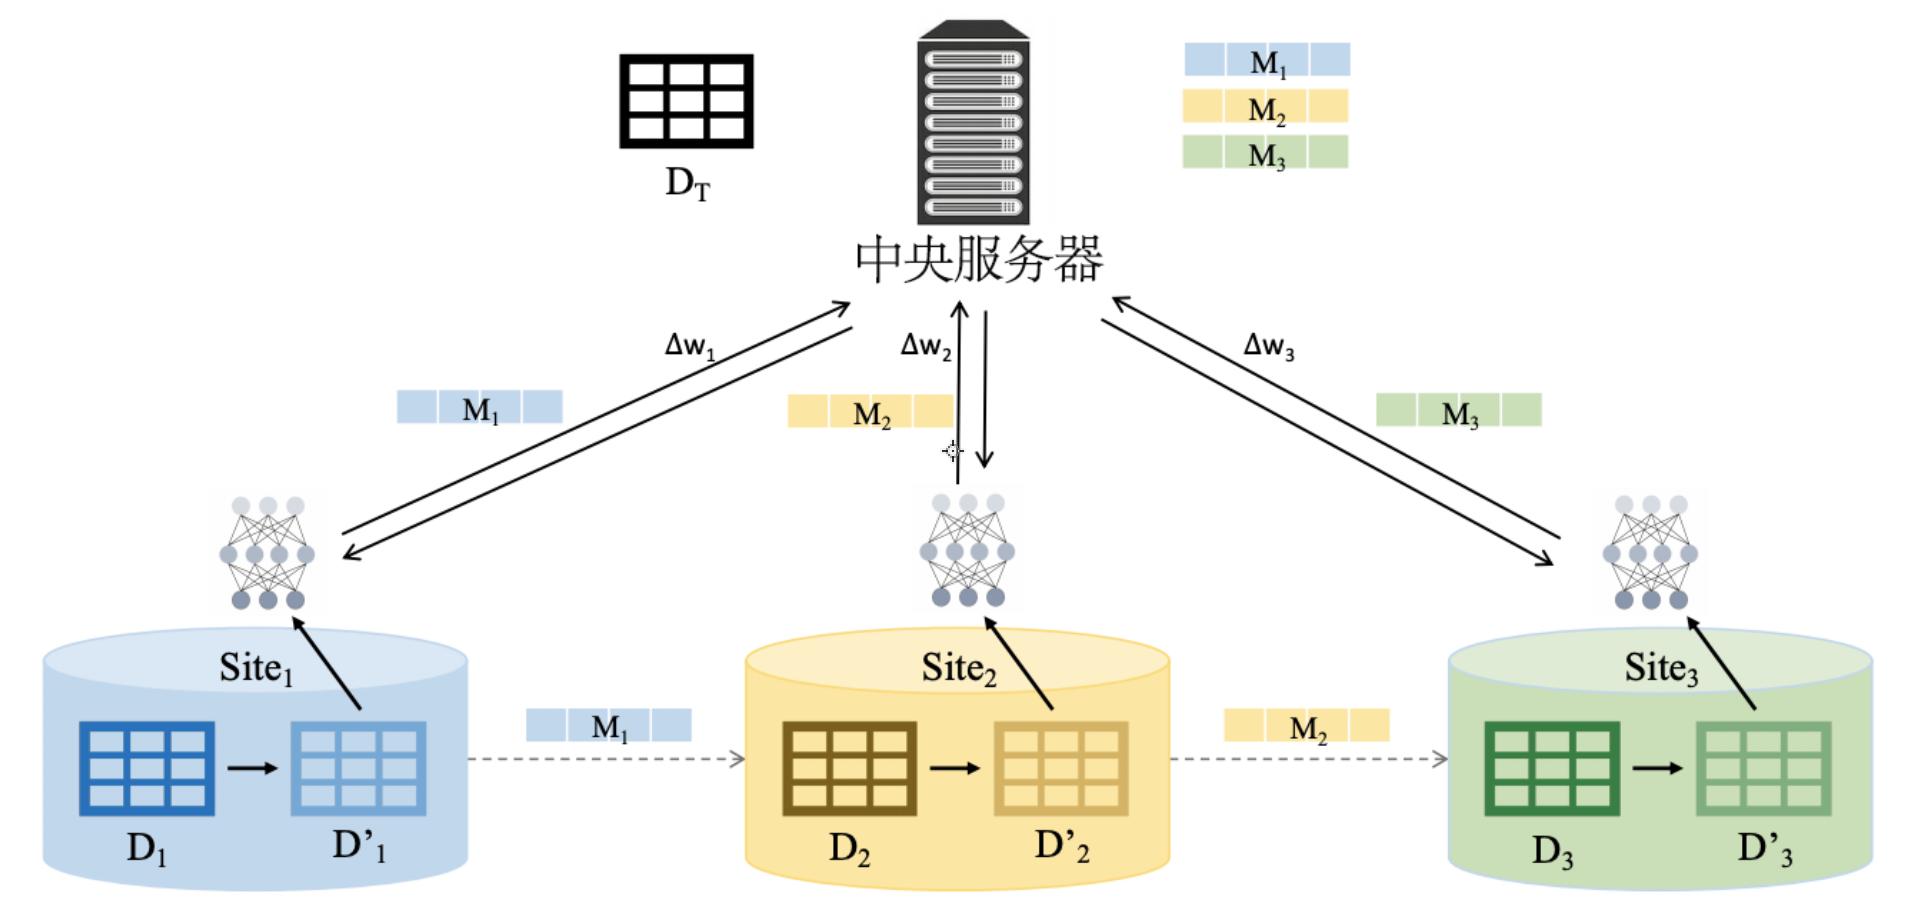
\includegraphics[scale=0.45]{fig2/C2/联邦学习模型流程}%联邦学习的系统架构
	\caption{联邦学习模型工作流程}
	\label{fig:联邦学习模型工作流程}	
\end{figure}

本文我们提出的方案是基于典型的分布式横向联邦学习系统架构,即各个本地参与者的样本空间相同,但是数据集特征不同。通过中央服务器,各个参与者相互协作,在保护个人本地敏感数据的同时,有效地提高本地学习效果。如图\ref{fig:联邦学习模型工作流程}所示,分布式横向联邦学习的基本工作流程如下:
\begin{itemize}
\item \textbf{初始化:}所有用户在他们的设备上都有一个预先分配的神经网络模型,并且可以自愿加入联邦学习协议,指定相同的深度学习和模型训练目标。
\item  \textbf{本地训练:}在一个给定的通信回合中,联邦学习参与者首先从中央服务器下载全局模型参数,然后在各自的本地数据集上进行模型训练,更新模型参数,之后将本地的参数更新上传到中央服务器。
\item \textbf{中央参数聚合:}中央服务器等待所有本地客户端将更新后的模型参数上传,聚合得到全局模型的参数,之后更新全局模型。
\item \textbf{迭代更新:}迭代地执行上述步骤直至全局模型参数满足收敛条件,最终得到最优的全局模型。
\end{itemize}{}

\section{神经网络}
\subsection{基本结构}
神经网络\upcite{ref34}最初的设计灵感来源于人脑的结构。我们知道,人类的大脑是处理信息的主要部分,也是人中枢神经系统中的重要部分。人脑中含有大量的神经元,它们像网状物一样复杂的相互连接。当人脑接收到外部环境或者感觉器官传入的刺激(兴奋),它随着神经元一层一层的将刺激(兴奋)传导到神经中枢(大脑或脊髓),神经中枢根据接收到的信号,作出不同的判断,最后传递到输出神经。
不同的信号,大脑都可以进行学习和分辨,而这一通用的模型,就是神经网络。

神经网络的基本组成单元是神经元,一个神经网络可能包含数百亿个简单的神经元,它们按层排列,密集而复杂的相互连接着。神经网络中每一层有多个神经元,层与层之间是“前馈传播”的,也就是说,网络中的数据只在一个方向上移动。一个单独的神经元可能与它前面一层的几个神经元相连,它从这些神经元接收数据;与它后面一层的几个神经元相连,它向这些神经元发送数据。每一层的神经元只有可能与其前一层和后一层的神经元相连接,不存在跨层连接。

\begin{figure}[!hbt]
\centering
	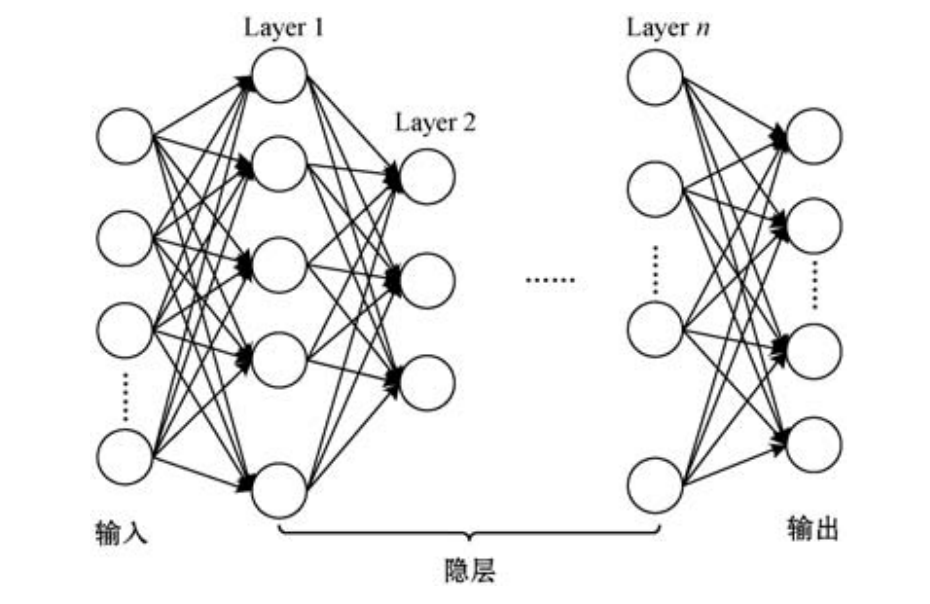
\includegraphics[scale=0.5]{fig2/C2/深度神经网络结构图}%联邦学习的系统架构
	\caption{神经网络结构图}
	\label{fig:神经网络结构图}	
\end{figure}

如图\ref{fig:神经网络结构图}所示,神经网络通常有三个部分:一个输入层、一个或多个隐藏层、一个输出层。输入层用于接收信息,当一个神经网络被训练时,其所有的权重和阈值最初都被设置为随机值,然后训练数据被送入输入层;之后传入隐藏层进行特征的提取、网络权重的调整使得隐藏层的神经单元对某种模式形成反应;最后传导到输出层,输出模型判断的结果。

\subsection{前向传播算法}

神经网络中层与层之间的” 前馈传播” 的算法简称为前向传播算法:网络中上一层的输出作为下一层的输入,并计算下一层的输出,一直到运算到输出层为止。如图\ref{fig:前馈神经网络结构图}所示,假设现有输入层的训练数据为$D=\left\{\left(x_{1}, y_{1}\right),\left(x_{2}, y_{2}\right), \cdots,\left(x_{m}, y_{m}\right)\right\}, x_{i} \in R^{d}, y_{i} \in R^{l}$,其中输入的样本包含$d$ 个属性,输出的向量是$l$维。

\begin{figure}[!hbt]
\centering
	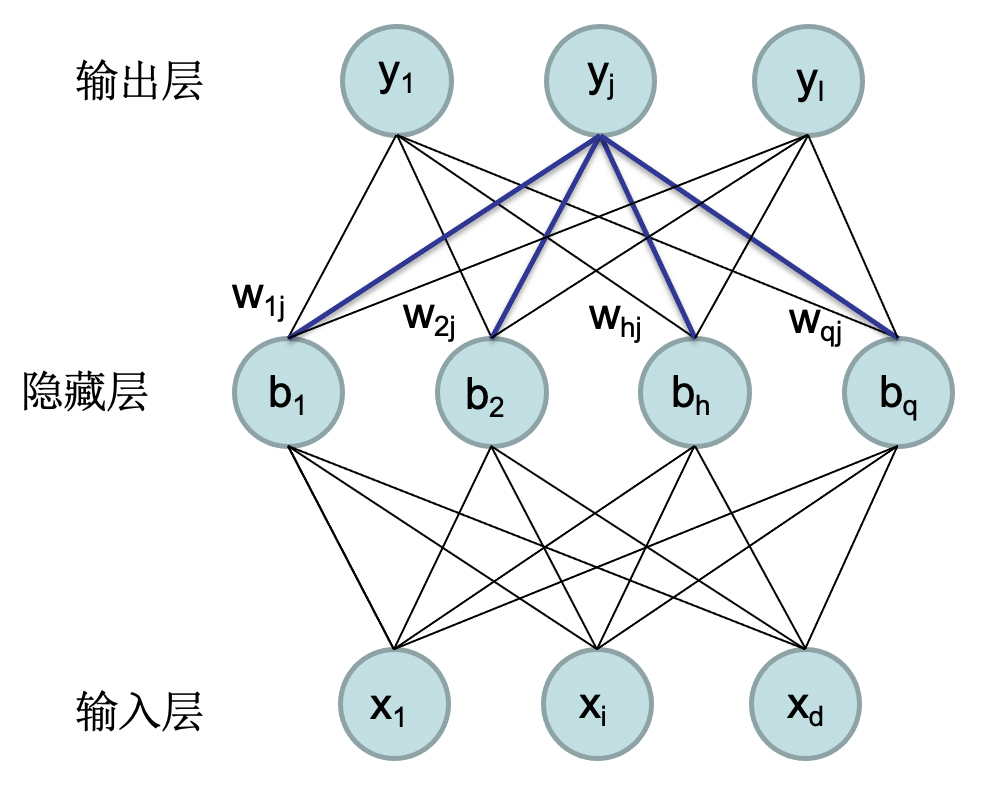
\includegraphics[scale=0.5]{fig2/C2/前馈神经网络}%
	\caption{前馈神经网络结构图}
	\label{fig:前馈神经网络结构图}	
\end{figure}

在此神经网络结构图中,假设隐藏层中神经元有$q$个,$\gamma_{h}$ 表示隐藏层第 $h$ 个神经元的阈值,$v_{i h}$表示隐藏层第$h$个神经元和输入层第$i$个神经元之间的连接权重,$w_{h j}$ 表示隐藏层第$h$个神经元和输出层第$j$个神经元之间的连接权重。输出层神经元的阈值用$\theta_{j}$ 表示。

隐藏层第 $h$ 个神经元接收到的输入为$\alpha_{h}=\sum_{i=1}^{d} v_{i h} x_{i}$,输出层第$j$个神经元接收到的输入为$\beta_{j}=\sum_{h=1}^{q} w_{h j} b_{h}$。其中 $b_{n}$ 为隐藏层第$h$ 个神经元的输出。
假设隐藏层和输出层神经元使用的激活函数为Sigmoid。对训练数据 $\left(x_{k}, y_{k}\right)$, 假定神经网络的输出为 $\hat{y}_{k}=\left(\hat{y}_{1}^{k}, \hat{y}_{2}^{k}, \cdots, \hat{y}_{l}^{k}\right)$, 即神经网络的预测输出表达式为:
\begin{equation}\label{神经网络预测输出}
\hat{y}_{j}^{k}=f\left(\beta_{j}-\theta_{j}\right)
\end{equation}

得到了神经网络预测的输出结果后,如何评估预测结果与真实值之间的差异大小呢?这里提出损失函数 $L$,比如采用均方差损失函数,这种损失是通过计算实际(目标)值和预测值之间的平方差的平均值,那么网络在样本集 $\left(x_{k}, y_{k}\right)$上的均方误差为:
\begin{equation}\label{神经网络损失函数}
E_{k}=\frac{1}{2} \sum_{j=1}^{l}\left(\hat{y}_{j}^{k}-y_{j}^{k}\right)^{2}
\end{equation}

\subsection{反向传播算法}
使用损失函数衡量得到预测值和真实值之间的差异程度后,接下来的想法是如何调整网络的权重和阈值使得最终的损失函数$L$值最小,也就是预测值最接近真实值,使得整个网络模型的结果最优。随机梯度下降(Stochastic Gradient Descent, SGD)算法是现有的比较经典的优化损失函数的算法。在每次迭代过程中,它通过批量随机抽取训练样本 ($B$),并计算损失函数 $L$ 的偏导数 $g_{B}=\frac{1}{|B|} \sum_{x \in B} \nabla_{\theta} L(\theta,$,$x$ ),然后沿着梯度的负方向 $-g_{B}$ 朝着局部最小值更新权重系数$\theta_{\circ}$,最小化损失函数。而在神经网络中,通常基于反向传播算法\upcite{ref29},实现梯度下降\upcite{ref30}策略。首先依据输出层的输出结果计算误差,再将误差反向传播到隐藏层神经元,最后依据隐层神经元的误差来对连接权重和阈值进行调整\upcite{ref31}。

总的来说,在深度神经网络中,对每个训练样本,通过前向传播算法从输入层、隐藏层到输出层依次训练,在输出层得到预测的结果,然后根据损失函数计算预测值与真实值之间的差异程度,之后根据反向传播算法调整权重系数,更新网络参数,使得损失函数的值最小,模型达到全局最优。

\section{差分隐私}
差分隐私最初是由微软研究院在2006年\upcite{ref9}针对统计数据库的隐私泄露问题提出的一种新的隐私定义,目的是使得数据库查询结果对于数据集中单个记录的变化不敏感。也就是说,单条记录的变化不会对查询结果产生明显的变化。那么攻击者就无法通过加入或减少一个记录,观察查询结果的变化来推测个体的具体信息。

差分隐私首先被应用于数据查询,为了更好地说明数据集之间的差异,定义了相邻数据集的概念:两个数据集只差一个信息或只差一个数值不同的记录\upcite{ref28}。因此,查询数据库相关信息的攻击者将无法以任何概率确定$X_{n}$是否存在于数据集中,而成员$X_{n}$被认为是相对安全的。

\subsection{基本定义}
\begin{define}[邻近数据集]\label{邻近数据集}
现有两个属性相近的数据集$D$和$D^{\prime}$,他们的数据记录差为$D \Delta D^{\prime}$,如果$\left|D \Delta D^{\prime}\right|=1$,则称数据集$D$和$D^{\prime}$为邻近数据集(Adjacent Dataset)。
\end{define}

\begin{figure}[!hbt]
\centering
	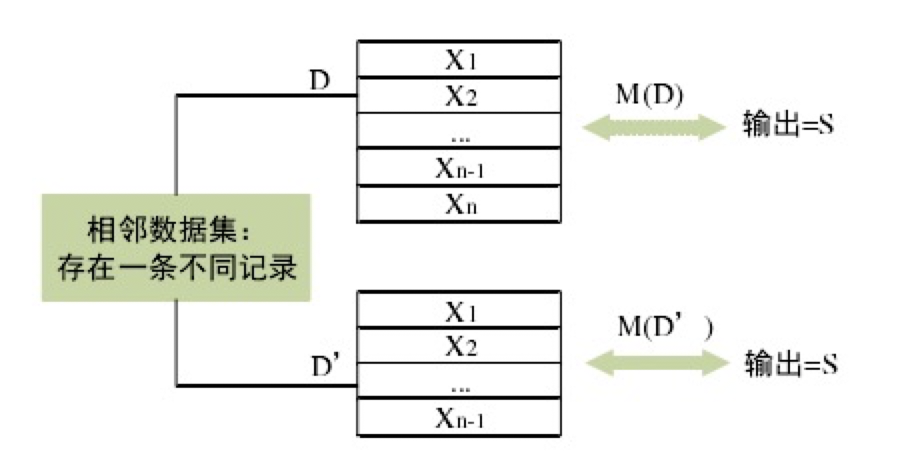
\includegraphics[scale=0.6]{fig2/C2/相邻数据集示意图}%联邦学习的系统架构
	\caption{差分隐私的相邻数据集示意图}
	\label{fig:相邻数据集示意图}	
\end{figure}

假设存在有限域 $Z,z \in Z$ 为 $Z$ 中的元素,从有限域 $Z$ 中抽样所得 $z$ 组成数据集 $D$,数据的维度为$d$,样本量为$n$。对数据集 $D$ 的查询即映射函数,用 $F=\left\{f_{1}, f_{2}, \cdots\right\}$ 来表示一组查询,算法 $M$ 表示满足差分隐私的查询机制,它通过对查询 $F$ 的结果进行处理,使之满足隐私保护的条件。

\begin{define}[差分隐私成立条件]\label{差分隐私成立条件}

若随机算法 $M: D \rightarrow R$ 满足 $(\varepsilon, \delta)-D P$,当且仅当相邻数据集 $d, d^{\prime}$ 对于算法 $M$ 的所有可能输出子集 $S \in R$ 满足不等式 $^{[40]}$ :
$$
\operatorname{Pr}[M(d) \in S] \leq e^{\varepsilon} \operatorname{Pr}\left[M\left(d^{\prime}\right) \in S\right]+\delta
$$
\end{define}
其中,$\varepsilon$ 表示隐私预算参数,$\varepsilon$ 越接近0代表着数据集$D$,$D^{\prime}$ 上输出的数据分布越接近,输出结果越不可区分,隐私预算越低,隐私保护的强度越高。添加值$\delta$表示$\varepsilon-\mathrm{DP}$ 的失败概率,是用于限制模型行为任意改变的概率,值通常选择小于 $1 /|D|$。当 $\delta=0$ 时转化为$\varepsilon-\mathrm{DP}$,这时候提供的隐私保护机制更为严格。


\subsection{相关概念}
差分隐私保护的实现是在查询函数的返回值中注入一定量的干扰噪声,但是注入的噪声量太大会影响最终结果的准确性,太少则无法保障数据的隐私性。那么如何衡量添加的噪声量,既能保障数据的安全,又能维持数据的可用性呢?这里针对数据集提出敏感度的概念,加入的噪声量大小与数据集的敏感度息息相关。对于相邻数据集$D$和$D^{\prime}$,他们的敏感度代表某一个查询函数在这两个相邻数据集上输出的最大不同。查询函数的类型决定了敏感度,也为噪声的添加提供了依据。

\begin{define}[全局敏感度]\label{全局敏感度}
假设存在函数 $f: D \rightarrow R^{d}$, 输入为一数据集,输出为$d$维的实数向量。 对于任意的邻近数据集 $D$ 和 $D^{\prime}$,
$$
G S_{f}=\max _{D, D^{\prime}}\left\|f(D)-f\left(D^{\prime}\right)\right\|_{1}
$$
称为函数 $f$ 的全局敏感度。
\end{define}

全局敏感度反映了一个查询函数在一对相邻数据集上进行查询时变化的最大范围,一般由查询函数本身决定。当全局敏感度太大,所生成的噪音可能会对数据进行过度保护,破坏了数据的可用性。

\begin{define}[局部敏感度]\label{局部敏感度}
对于一个查询函数 $f_{:} D \rightarrow R^{d}$, 其中 $D$ 为一个数据集, $R^{d}$为d维实数向量,是查询的返回结果。对于数据集D存在邻近数据集 $D^{\prime}$, 查询函数$f$在数据集$D$ 上的局部敏感度定义为:
$L S_{f}(D)=\max _{D^{\prime}}\left\|f(D)-f\left(D^{\prime}\right)\right\|_{1}$。
\end{define}

由于局部敏感度只是对于一个数据集做变化,利用了数据集的数据分布特征,局部敏感度通常要比全局敏感度小得多。但是,也正是因为局部敏感度在某种程度上反映了数据集的分布特征,所以直接应用局部敏感度生成噪声可能会泄漏数据的隐私信息。

在解决一个复杂的差分隐私保护问题时,可能在多个场景,多个步骤多次应用差分隐私技术,在这种情况下,如何保证最终结果的差分隐私性,以及隐私保护的程度该如何去度量呢?这里引出差分隐私的三个最重要的性质:可量化性、可组合性和后处理不变性\upcite{ref35}。

可量化性指的是差分隐私算法在计算特定随机化过程时,可以透明化、精准量化所施加的噪声大小,即上文提及的隐私预算。这样使用者就可以清楚地知道算法的隐私保护力度;差分隐私的后处理不变性,确保了即使对算法的结果进行进一步处理,只要不引入额外信息,后续的处理就并不会削弱算法的隐私保护力度。组合性是指将独立的满足差分隐私的算法进行串行组合或者并行组合之后得到的算法依然满足差分隐私。

\begin{theorem}[串行组合]\label{串行组合}
给定 $\mathbf{n}$ 个随机算法 $M_{i}(1 \leq i \leq n)$ 满足 $\varepsilon_{i}-DP$, 那么针对一个数据库 $D$ 而言, 在 $\mathrm{D}$ 上的算法串行序列组合满足$\varepsilon-\mathrm{DP}$, 其中 $\sum_{i=1}^{n} \varepsilon_{i}=\varepsilon$ 。
\end{theorem}

\begin{theorem}[并行组合]\label{并行组合}
如果数据库 $\mathrm{D}$, 划分成 $\mathrm{n}$ 个不相交的子集 $\left\{\mathrm{D}_{1}, \mathrm{D}_{2}, \ldots, \mathrm{D}_{n}\right\}$, 在每个子集上应用满足$\varepsilon_{i}-\mathrm{DP}$的算法 $\mathrm{M}_{i}$,  那么在$\left\{\mathrm{D}_{1}, \mathrm{D}_{2}, \ldots, \mathrm{D}_{n}\right\}$ 上整体满足 $\left(\max \left\{\varepsilon_{1}, \ldots, \varepsilon_{n}\right\}\right)-\mathrm{DP}$。
\end{theorem}

通过差分隐私的串并行组合定理,人们可以利用基础的差分隐私算法设计出复杂的满足差分隐私的系统,只要算法中的每一个步骤都满足差分隐私要求,那么这个算法的最终结果将满足差分隐私特性,这也是差分隐私的重要优势之一。 

\subsection{实现机制}
在差分隐私的实际应用中,如何针对不同的场景和问题设计添加噪声的机制使算法能满足差分隐私保护的要求呢?差分隐私的实现机制主要分为拉普拉斯机制(Lapalace Mechanism)\upcite{ref9}、指数机制(Exponential Mechanism)\upcite{ref32}与高斯机制(Gaussian Mechanism)\upcite{ref33}。其中,指数机制适用于非数值型结果的隐私保护,拉普拉斯机制和高斯机制适用于对数值型结果的隐私保护\upcite{ref35}。

\begin{theorem}[拉普拉斯机制]\label{拉普拉斯机制}
一个查询函数 $f: D \rightarrow R$, 机制 $M$ 满足 $\varepsilon-D P$, 当:
$$
M(D)=f(D)+\operatorname{Lap}\left(\frac{\Delta f}{\varepsilon}\right)
$$
\end{theorem}
其中,噪声参数满足$\frac{\Delta f}{\varepsilon}$ 的 Laplace 分布。

与拉普拉斯机制类似,高斯机制对输入的所有维度添加高斯噪声干扰 $N\left(0,\sigma^{2}\right)$。
\begin{theorem}[高斯机制]\label{高斯机制}
对任意 $\epsilon \in(0,1), \delta>(\sqrt{2 \ln (1.25 / \delta) f} / \epsilon)$, 有噪音 $Y \sim N\left(0, \delta^{2}\right)$,则满足 $(\epsilon, \delta)$-差分隐私。
$$
\operatorname{Pr}\left[\mathscr{A}\left(D_{1}\right)=\tilde{D}\right] \leq e^{\epsilon} \times \operatorname{Pr}\left[\mathscr{A}\left(D_{2}\right)=\tilde{D}\right]+\delta
$$
\end{theorem}

其中, $\epsilon$ 表示隐私保护预算, $\delta$ 表示隐私保护的水平误差, 是一个较小的常数。

但是对于离散型的查询结果或数据要如何处理呢?这就产生了指数机制,通常使用指数机制来随机选择离散的输出结果来满足差分隐私。指数机制整体的思想就是,对于一个查询函数,不是确定性的输出一个$R_{i}$结果,而是以一定的概率值返回结果,从而实现差分隐私。

\begin{theorem}[指数机制]\label{指数机制}
指数机制满足差分隐私, 如果:
$$
A(D,u)=\left\{p: \mid \operatorname{Pr}[p \in O] \propto \exp \left(\frac{\varepsilon u(D,p)}{2 \Delta u}\right)\right\}
$$
\end{theorem}
其中 $u(D,p)$为评分函数,评分越高,则输出的概率越大\upcite{ref53},$\Delta u$表示$u(D,p)$的全局敏感度。

\section{本章小结}
本章节为基础知识,对于论文的研究所涉及的基础知识定理进行了讲解。本章主要介绍了神经网络的结构和算法、联邦学习系统的学习协议以及差分隐私的基本概念、定义和定理。分布式联邦学习系统是本论文主要使用的系统架构,本文所针对的攻击模型和隐私保护方案都是基于该分布式联邦学习系统。

